\documentclass{beamer}
\usetheme{Berlin}  %% Themenwahl
\usecolortheme{beaver}

\usepackage{listings}
\usepackage{graphicx}
\usepackage{hyperref}
\usepackage[utf8]{inputenc}
\usepackage{amssymb}
\usepackage{amsmath}
\usepackage{esvect}
%\usepackage{mcode}
 
\title{Ray Tracing Optimization}
\author{Kashofer, Radschek, Wagner}
\date{\today}

%\section{Foliensection}
%\begin{frame} %%Eine Folie
%	\frametitle{Folientitel} %%Folientitel
%	Das ist eine Dummy-Section
%\end{frame}

\begin{document}
\maketitle
\frame{\tableofcontents[currentsection]}
 
\section{Profiling}
\begin{frame} %%Eine Folie
	\frametitle{Rendering time} %%Folientitel
  	\begin{itemize}
		\item original code: $45 \dfrac{sec}{Frame}$
		\item simple C-Code adaptions: $43 \dfrac{sec}{Frame}$
		\item replaced fix\_mul16 by ci\_mul looped functions: $36 \dfrac{sec}{Frame}$
		\item fix\_mul16 calls ci\_mul: $17 \dfrac{sec}{Frame}$
	\end{itemize}
	$\quad$\\
	$\rightarrow$ Transition looped functions from SW to HW to achieve target speed
\end{frame}

\begin{frame} %%Eine Folie
	\frametitle{Algorithm} %%Folientitel
  	\begin{figure}
		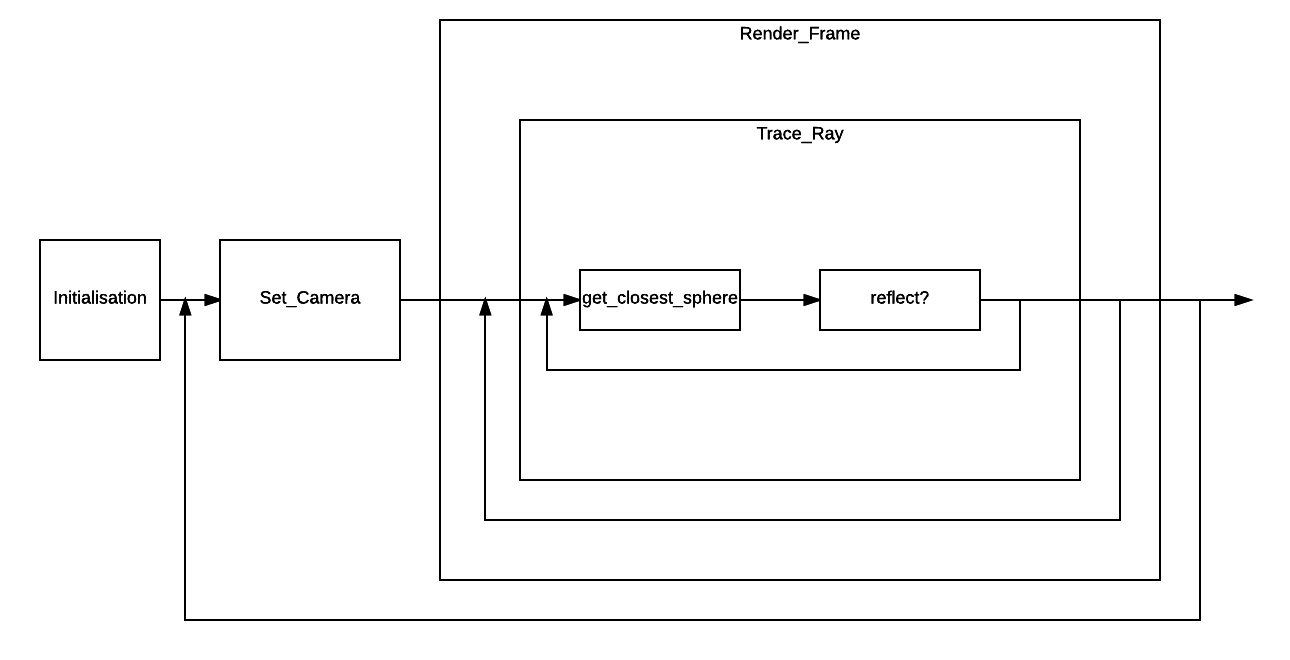
\includegraphics[width=\textwidth]{algo.png}
		\caption{Schematic of the algorithm}
	\label{fig1}
	\end{figure}
\end{frame}


\begin{frame} %%Eine Folie
	\frametitle{Functions} %%Folientitel
  	\begin{itemize}
		\item Initialisation: once in entire algorithm
		\item SetCamera: once every frame
		\item GetClosestSphere: up to REFLECT times per ray
		\item Reflect: up to REFLECT times per ray
	\end{itemize}
\end{frame}



\section{Optimization}
\begin{frame} %%Eine Folie
	\frametitle{Outline}
	Idea: automate entire frame-rendering
\end{frame}

\section{Optimization}
\begin{frame} %%Eine Folie
	\frametitle{Overview} %%Folientitel
	Lorem ipsum
\end{frame}

\begin{frame} %%Eine Folie
	\frametitle{Details} %%Folientitel
	Lorem ipsum
\end{frame}

\section{Future tasks}
\begin{frame} %%Eine Folie
	\frametitle{Details} %%Folientitel
	Set dolor
\end{frame}

\end{document}